\subsubsection{UC 3 - Operazioni disponibili nella \texttt{\textit{Homepage} Agenti} 
               autenticati come clienti}
\begin{figure}[H]
    \vspace{2em}
    \centering
    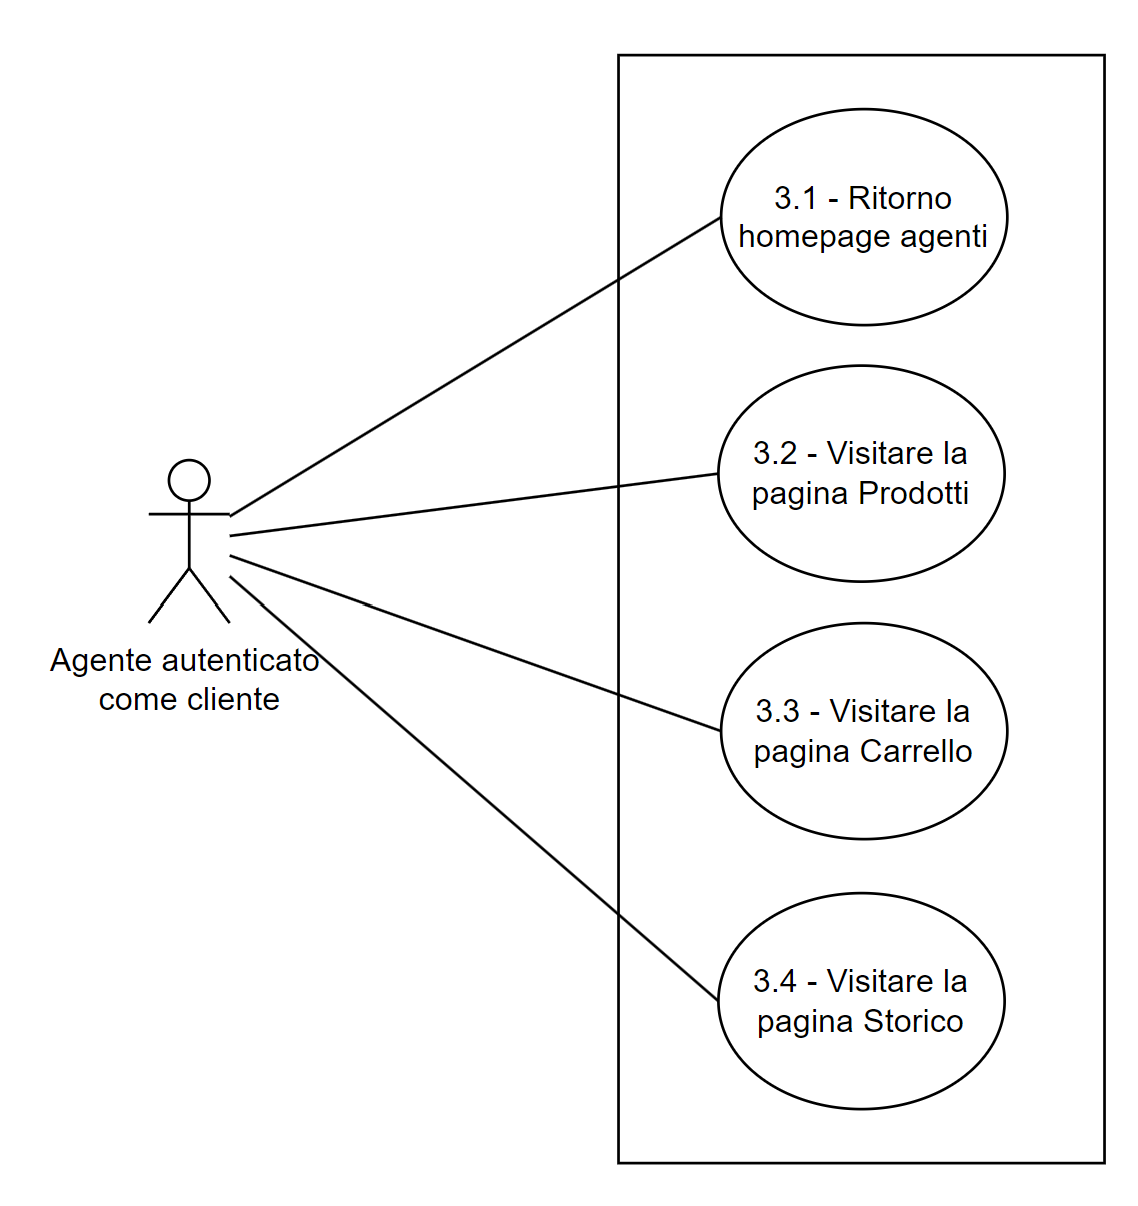
\includegraphics[width=0.75\columnwidth]{img/usecase/UC 3.png}
    \caption{\textit{Use Case} 3: Operazioni disponibili nella \texttt{\texttt{\textit{Homepage} Agenti}}}
    \label{fig:uc_3}
\end{figure}

\begin{usecase}{ 3.1}{Ritorno \texttt{\textit{Homepage} Agenti}}
    \usecaseactors{Agente.}
    \usecasedesc{L'agente, cliccando nell'apposito menu il pulsante "\textit{Homepage} Agenti", ritorna alla 
                 \texttt{\textit{Homepage} Agenti}.}
    \usecasepre{L'agente ha selezionato un cliente dalla lista.}
    \usecasepost{L'agente si è spostato nella \texttt{\textit{Homepage} Agenti}.}
    \usecasescen{
        \begin{itemize}
            \item L'agente seleziona un cliente della lista;
            \item L'agente viene spostato nella \textit{\texttt{Homepage}};
            \item L'agente può operare nell'\textit{app} come il cliente selezionato;
            \item L'agente preme il pulsante "\textit{Homepage} Agenti";
            \item L'agente ritorna alla \texttt{\textit{Homepage} Agenti}.
        \end{itemize}}
    \label{uc:uc_3.1}
\end{usecase}

\begin{usecase}{ 3.2}{Visitare la pagina \texttt{Prodotti}}
    \usecaseactors{Agente.}
    \usecasedesc{L'agente, cliccando nell'apposito menu il pulsante "Prodotti", può operare nella pagina 
                 \texttt{Prodotti} come il cliente selezionato.}
    \usecasepre{L'agente ha selezionato un cliente dalla lista.}
    \usecasepost{L'agente si è spostato nella pagina \texttt{Prodotti}.}
    \usecasescen{
        \begin{itemize}
            \item L'agente seleziona un cliente della lista;
            \item L'agente viene spostato nella \textit{\texttt{Homepage}};
            \item L'agente preme il pulsante "Prodotti";
            \item L'agente viene spostato nella pagina \texttt{Prodotti} dove può operare come il cliente selezionato.
        \end{itemize}}
    \label{uc:uc_3.2}
\end{usecase}

\begin{usecase}{ 3.3}{Visitare la pagina \texttt{Carrello}}
    \usecaseactors{Agente.}
    \usecasedesc{L'agente, cliccando nell'apposito menu il pulsante "Carrello", può operare nella pagina 
                 \texttt{Carrello} come il cliente selezionato.}
    \usecasepre{L'agente ha selezionato un cliente dalla lista.}
    \usecasepost{L'agente si è spostato nella pagina \texttt{Carrello}.}
    \usecasescen{
        \begin{itemize}
            \item L'agente seleziona un cliente della lista;
            \item L'agente viene spostato nella \textit{\texttt{Homepage}};
            \item L'agente preme il pulsante "Carrello";
            \item L'agente viene spostato nella pagina \texttt{Carrello} dove può operare come il cliente selezionato.
        \end{itemize}}
    \label{uc:uc_3.3}
\end{usecase}

\begin{usecase}{ 3.4}{Visitare la pagina \texttt{Storico}}
    \usecaseactors{Agente.}
    \usecasedesc{L'agente, cliccando nell'apposito menu il pulsante "Storico", può operare nella pagina 
                 \texttt{Storico} come il cliente selezionato.}
    \usecasepre{L'agente ha selezionato un cliente dalla lista.}
    \usecasepost{L'agente si è spostato nella pagina \texttt{Storico}.}
    \usecasescen{
        \begin{itemize}
            \item L'agente seleziona un cliente della lista;
            \item L'agente viene spostato nella \textit{\texttt{Homepage}};
            \item L'agente preme il pulsante "Storico";
            \item L'agente viene spostato nella pagina \texttt{Storico} dove può operare come il cliente selezionato.
        \end{itemize}}
    \label{uc:uc_3.4}
\end{usecase}